% Options for packages loaded elsewhere
\PassOptionsToPackage{unicode}{hyperref}
\PassOptionsToPackage{hyphens}{url}
%
\documentclass[
  a4paper,
]{scrbook}

\usepackage{amsmath,amssymb}
\usepackage{iftex}
\ifPDFTeX
  \usepackage[T1]{fontenc}
  \usepackage[utf8]{inputenc}
  \usepackage{textcomp} % provide euro and other symbols
\else % if luatex or xetex
  \usepackage{unicode-math}
  \defaultfontfeatures{Scale=MatchLowercase}
  \defaultfontfeatures[\rmfamily]{Ligatures=TeX,Scale=1}
\fi
\usepackage{lmodern}
\ifPDFTeX\else  
    % xetex/luatex font selection
  \setmainfont[]{Latin Modern Roman}
  \setsansfont[]{Latin Modern Roman}
\fi
% Use upquote if available, for straight quotes in verbatim environments
\IfFileExists{upquote.sty}{\usepackage{upquote}}{}
\IfFileExists{microtype.sty}{% use microtype if available
  \usepackage[]{microtype}
  \UseMicrotypeSet[protrusion]{basicmath} % disable protrusion for tt fonts
}{}
\makeatletter
\@ifundefined{KOMAClassName}{% if non-KOMA class
  \IfFileExists{parskip.sty}{%
    \usepackage{parskip}
  }{% else
    \setlength{\parindent}{0pt}
    \setlength{\parskip}{6pt plus 2pt minus 1pt}}
}{% if KOMA class
  \KOMAoptions{parskip=half}}
\makeatother
\usepackage{xcolor}
\setlength{\emergencystretch}{3em} % prevent overfull lines
\setcounter{secnumdepth}{5}
% Make \paragraph and \subparagraph free-standing
\ifx\paragraph\undefined\else
  \let\oldparagraph\paragraph
  \renewcommand{\paragraph}[1]{\oldparagraph{#1}\mbox{}}
\fi
\ifx\subparagraph\undefined\else
  \let\oldsubparagraph\subparagraph
  \renewcommand{\subparagraph}[1]{\oldsubparagraph{#1}\mbox{}}
\fi


\providecommand{\tightlist}{%
  \setlength{\itemsep}{0pt}\setlength{\parskip}{0pt}}\usepackage{longtable,booktabs,array}
\usepackage{calc} % for calculating minipage widths
% Correct order of tables after \paragraph or \subparagraph
\usepackage{etoolbox}
\makeatletter
\patchcmd\longtable{\par}{\if@noskipsec\mbox{}\fi\par}{}{}
\makeatother
% Allow footnotes in longtable head/foot
\IfFileExists{footnotehyper.sty}{\usepackage{footnotehyper}}{\usepackage{footnote}}
\makesavenoteenv{longtable}
\usepackage{graphicx}
\makeatletter
\def\maxwidth{\ifdim\Gin@nat@width>\linewidth\linewidth\else\Gin@nat@width\fi}
\def\maxheight{\ifdim\Gin@nat@height>\textheight\textheight\else\Gin@nat@height\fi}
\makeatother
% Scale images if necessary, so that they will not overflow the page
% margins by default, and it is still possible to overwrite the defaults
% using explicit options in \includegraphics[width, height, ...]{}
\setkeys{Gin}{width=\maxwidth,height=\maxheight,keepaspectratio}
% Set default figure placement to htbp
\makeatletter
\def\fps@figure{htbp}
\makeatother

\usepackage{booktabs}
\usepackage{longtable}
\usepackage{array}
\usepackage{multirow}
\usepackage{wrapfig}
\usepackage{float}
\usepackage{colortbl}
\usepackage{pdflscape}
\usepackage{tabu}
\usepackage{threeparttable}
\usepackage{threeparttablex}
\usepackage[normalem]{ulem}
\usepackage{makecell}
\usepackage{xcolor}
\usepackage{fancyhdr}
\usepackage{titling}
\setlength{\droptitle}{-2cm}
\preauthor{
  \begin{center}
  \Large
  \vspace{10mm}
  by
  \vspace{20mm}
}
\postauthor{
  \end{center}
  \vfill
}

\predate{
  \begin{center}
  A thesis 
  submitted in partial fulfilment of the \\
  requirements of the degree of \\
  Doctor of Philosophy in Physics\\               % Degree
  School of Physical and Chemical Sciences\\          % Department
  Te Herenga Waka - Victoria University of Wellington\\                       % University 
  \vspace{5mm}
}
\postdate{
  \\
  
\includegraphics[width=3in,height=1.5in]{figures/VUW-logo.png}\\
  \end{center}
  }

\renewcommand{\topfraction}{.8}
\renewcommand{\floatpagefraction}{.8}
\clubpenalty=9996
\widowpenalty=9999
\makeatletter
\makeatother
\makeatletter
\@ifpackageloaded{bookmark}{}{\usepackage{bookmark}}
\makeatother
\makeatletter
\@ifpackageloaded{caption}{}{\usepackage{caption}}
\AtBeginDocument{%
\ifdefined\contentsname
  \renewcommand*\contentsname{Table of contents}
\else
  \newcommand\contentsname{Table of contents}
\fi
\ifdefined\listfigurename
  \renewcommand*\listfigurename{List of Figures}
\else
  \newcommand\listfigurename{List of Figures}
\fi
\ifdefined\listtablename
  \renewcommand*\listtablename{List of Tables}
\else
  \newcommand\listtablename{List of Tables}
\fi
\ifdefined\figurename
  \renewcommand*\figurename{Figure}
\else
  \newcommand\figurename{Figure}
\fi
\ifdefined\tablename
  \renewcommand*\tablename{Table}
\else
  \newcommand\tablename{Table}
\fi
}
\@ifpackageloaded{float}{}{\usepackage{float}}
\floatstyle{ruled}
\@ifundefined{c@chapter}{\newfloat{codelisting}{h}{lop}}{\newfloat{codelisting}{h}{lop}[chapter]}
\floatname{codelisting}{Listing}
\newcommand*\listoflistings{\listof{codelisting}{List of Listings}}
\makeatother
\makeatletter
\@ifpackageloaded{caption}{}{\usepackage{caption}}
\@ifpackageloaded{subcaption}{}{\usepackage{subcaption}}
\makeatother
\makeatletter
\@ifpackageloaded{tcolorbox}{}{\usepackage[skins,breakable]{tcolorbox}}
\makeatother
\makeatletter
\@ifundefined{shadecolor}{\definecolor{shadecolor}{rgb}{.97, .97, .97}}
\makeatother
\makeatletter
\makeatother
\makeatletter
\makeatother
\ifLuaTeX
  \usepackage{selnolig}  % disable illegal ligatures
\fi
\usepackage[citestyle = ieee,urldate = iso8601]{biblatex}
\addbibresource{references.bib}
\IfFileExists{bookmark.sty}{\usepackage{bookmark}}{\usepackage{hyperref}}
\IfFileExists{xurl.sty}{\usepackage{xurl}}{} % add URL line breaks if available
\urlstyle{same} % disable monospaced font for URLs
\hypersetup{
  pdftitle={Developing an Insect Odorant Receptor Bioelectronic Nose for Vapour-Phase Detection},
  pdfauthor={Eddyn Oswald Perkins Treacher},
  hidelinks,
  pdfcreator={LaTeX via pandoc}}

\title{Developing an Insect Odorant Receptor Bioelectronic Nose for
Vapour-Phase Detection}
\author{Eddyn Oswald Perkins Treacher}
\date{Oct 2024}

\begin{document}
\frontmatter

\maketitle

\clearpage
\newpage
\thispagestyle{empty} % Hide header and footer on this page
\mbox{~}
\clearpage
\newpage

%----------------------------------------------
%   Abstract
%----------------------------------------------

\thispagestyle{plain}

\begin{flushleft}
% Manually add a section to the table of contents
\pagenumbering{roman}
\addcontentsline{toc}{chapter}{Abstract}
\huge\textbf{Abstract}
\end{flushleft}

\vspace*{\baselineskip}

The ability to detect volatile organic compounds in a highly sensitive and selective manner is desirable for applications as varied as diagnosis of illnesses at a remote clinic, monitoring of air in an industrial setting, or identification of invasive organisms at a biosecurity checkpoint. Historically, animal noses have been used for such tasks, as their combined sensitivity and selectivity are greatly superior to traditional artificial sensors. However, training and deploying animals in such situations is both time and cost intensive. In recent years, an improved understanding of \textit{in vivo} biological sensing has led to efforts to mimic these highly efficient processes in an artificial sensor format. \\[5pt] To this end, a “bioelectronic nose” was developed. This sensor uses an artificial transducer to amplify responses of an insect olfactory system to specific volatile compounds. Thin-film transistors were used as the amplifier element, given their low cost, small size and extreme sensitivity. Various thin-film morphologies were compared, and their suitability for bioelectronic nose development assessed. Transducers made using a novel steam-assisted thin-film deposition technique were found to have highly consistent device-to-device electrical properties relative to other films. Films made using this process typically showed more surface contamination than other morphologies, but their high sensitivity was nonetheless confirmed with a non-specific sensing series in an aqueous environment. \\[5pt] One of the major challenges encountered in this thesis was variability in the quality of sensor functionalisation. Raman spectroscopy and fluorescence microscopy confirmed an existing non-covalent attachment method could successfully immobilise nanodiscs onto the transistor channel region. However, various sensors functionalised using the same procedure often exhibited no sensing activity. Extensive electrical characterisation indicated the presence of an unidentified contamination layer preventing electrical interaction between the insect odorant receptors and transducer thin-film. It was shown that this layer was unlikely to be directly associated with the thin-film morphology used for the transducer. \\[5pt] Subsequently, an alternative biotin-based non-covalent method which eliminated several possible contamination sources was trialled. This alternative biotin-based method was used to demonstrate successful aqueous sensing of femtomolar concentrations of methyl salicylate by an iOR10a-functionalised device. When tested in a custom-built vapour delivery system, a similar bioelectronic sensor was shown to be highly sensitive to the target vapour. However, consistent reproduction of the biotin-based method was challenging due to the invasive cleaning method involved. It was therefore difficult to determine conclusively whether sensor responses were selective. By finding new, systematic approaches to address the major barriers to sensor success carefully identified in this work, there are promising signs that a highly reliable vapour-phase bioelectronic nose can be produced.

%\fancyhf{} %clear all headers and footers fields
%\thispagestyle{fancy} % Change header and footer on this page
%\renewcommand{\headrulewidth}{0pt}
%\fancyhead[L]{\textit{Abstract}} % Set header content
%\fancyfoot[L]{\thepage} %prints the page number on the right side of the header

\clearpage
\newpage
\thispagestyle{empty} % Hide header and footer on this page
\mbox{~}
\clearpage
\newpage


%----------------------------------------------
%   Acknowledgement
%----------------------------------------------

\thispagestyle{plain}

\begin{flushleft}
% Manually add a section to the table of contents
\addcontentsline{toc}{chapter}{Acknowledgements}
\huge\textbf{Acknowledgements}
\end{flushleft}

\vspace*{\baselineskip}

I would first like to acknowledge the lands of my ancestors, and the lands of the sovereign first peoples to which my ancestors travelled.\\[5pt]
\textit{Noon of Essex to Warrang, on the Friends, Autumn 1811} \\[5pt]
\textit{Cave of Cambridgeshire to Warrang, on the Royal Charlotte, Autumn 1825} \\[5pt]
\textit{Boyce of Suffolk to Warrang, 1832} \\[5pt] 
\textit{Charlton of Northumberland to Warrang, on the Clyde, Spring 1834} \\[5pt]
\textit{Prouse of Devonshire to Pito-one, on the Duke of Roxburgh, Summer 1840} \\[5pt]
\textit{Ebden of Devonshire to Pito-one, on the Tyne, Winter 1841} \\[5pt]
\textit{Collis of Hampshire to Pito-one, on the Birman, Autumn 1842} \\[5pt]
\textit{Swann of Loch Garman to Te Whanganui-a-Tara, 1844} \\[5pt] 
\textit{Blythe of Berkshire to Whakatū, circa 1846} \\[5pt]
\textit{Innes of Berkshire to Naarm, on the Sacramento, Autumn 1853} \\[5pt]
\textit{Sheppard of Gloucestershire to Naarm, 1853} \\[5pt] 
\textit{Bruce of London to Naarm, on the Omega, Autumn 1855} \\[5pt]
\textit{Quennell of Surrey to Warrang, on the Asiatic, Winter 1855} \\[5pt]
\textit{Barr of Glasgow to Kōpūtai, on the Sir Edward Paget, Winter 1856} \\[5pt] 
\textit{Perkins of London to Te Whanganui-a-Tara, on the Matoaka, Spring 1859} \\[5pt]
\textit{McKee of Antrim to Tāmaki Makaurau, on the Indian Empire, Spring 1862} \\[5pt]
\textit{Sandilands of Peeblesshire to Ōtepoti, circa 1864} \\[5pt] 
\textit{Treacher of Berkshire to Te Whanganui-a-Tara, on the Wild Duck, Summer 1865} \\[5pt]
\textit{McTaggart of Argyllshire to Kōpūtai, on the Edward P. Bouverie, Autumn 1869} \\[5pt] 
\textit{Chapman of Kent to Whakatū, on the Adamant, Winter 1874} \\[5pt]
\textit{Cheel of London to Whakatū, on the Queen Bee, Winter 1877} \\[5pt]  
\textit{Hutchison of Aberdeen to Tarntanya, before 1882.} \\[5pt] 
I chose to start my doctoral studies just a few months into a global pandemic. Completing a challenging project with a worldwide crisis in the background might have been impossible without the supervision of AProf. Natalie Plank. Her ability to adapt to and overcome any problem has taught me that there is no situation which is truly unmanageable. I am deeply grateful for her leadership throughout a time of particular chaos. \\[5pt] I started this project with minimal formal training in biological science, coming from a primarily physics and engineering background. 
\newpage
\fancyhf{} %clear all headers and footers fields
\thispagestyle{fancy} % Change header and footer on this page
\renewcommand{\headrulewidth}{0pt}
\fancyhead[L]{\textit{Acknowledgements}} % Set header content
\fancyfoot[L]{\thepage} %prints the page number on the left side of the header
The immense support I received from Melissa Jordan and Colm Carraher from the Institute for Plant and Food Research (PFR) to complete this project meant that this was not an issue, and I thank them both immensely for this. \\[5pt] I would not have been able to begin this thesis without the financial backing and support I received from PFR and the Better Border Biosecurity (B3) programme. In particular, I am very grateful to Andrew Kralicek, formerly with PFR and now at Scentian Bio, and the ex-Director of B3, David Teulon, for helping to secure funding for my project. I would also like to thank the donor of the Ernest Marsden Scholarship in Physics for their significant financial support. \\[5pt] There are many incredibly supportive people who I worked alongside during my project. I would like to start off by thanking Rifat Ullah, whose mentoring and kindness encouraged me to pursue further study. His work on the initial design and setup of the vapour delivery system was invaluable to me throughout this project. I am also especially grateful to Alex Puglisi, for constructing the mechanical elements of the vapour delivery system and giving me extensive feedback on the system design. I would like to thank Peter Coard, for his advice and guidance when constructing the electrical elements of the vapour delivery system. I would also like to thank Selvan Murugathas for his advice on constructing the insect odorant receptor sensors, as well as Damon Colbert and Valentina Lucarelli, who provided the insect odorant receptor nanodiscs used in this work. \\[5pt] Thank you to AProf. Ben Ruck, my supportive secondary supervisor, and to AProf. Franck Natali, for always asking about my thesis in the tearoom. Thank you to Gideon Gouws for his friendly encouragement and advice. For their substantial technical assistance and mentoring during this project, I would also like to thank Alan Rennie, Grant Franklin, Chris Lepper, Rashika Gunasekara, Pete Jebson and Sushila Pillai from VUW, Andrew Chan from PFR, AProf. Charles Unsworth from the University of Auckland, and Prof. Simon Brown and his nanomaterials group from the University of Canterbury. \\[5pt] I was lucky enough to start my doctoral program just as a group of supportive and talented senior students were finishing, and finished just as a group of enthusiastic and talented new doctoral students were starting. A special thanks to Jenna Nyugen, Erica Happe and Erica Cassie for teaching me the fabrication processes and characterisation procedures that made this thesis happen; and a special thanks to Marissa Dierkes, Danica Fontein, Sangar Begzaad and Alireza Zare, for their incredible support throughout the thesis writing process. \\[5pt] I would further like to thank everyone else I shared an office with and worked alongside, including Jackson, Will, Roshni, Ali, Kira, Catherine, Martin, Janani, Ted, Kiri and Joe. I would also like to thank all the interns and summer students who I worked with during this project. \\[5pt] A massive thank you to Openstar Technologies. It has been an honour to work on a cutting-edge plasma physics project right here in Wellington. A particularly big thank you to Ratu, Darren, Thomas, Ben and Gabriel for having me as part of the team. Thank you also to the other Openstar interns, in particular the other physics interns, Valentina and Benjy. I sincerely hope to see fusion with net energy gain in Aotearoa New Zealand within the next decade. \\[5pt] I want to thank Shodokan Aikido New Zealand for their support throughout this thesis, in particular for the once-in-a-lifetime opportunity to travel to Osaka to be graded for first-dan by Nariyama Shihan. Thanks for all the training and support, Ian. Thank you to all the friends and family, old and new, who have supported me over these wild past few years. You know who you are. \\[5pt] Thank you to my brother, Keeson, and to my parents, Hilary and Phillip. Your support means everything to me, and I would not be where I am today without you. Our Friday lunchtime cafe visits inspired and motivated me throughout the doctoral program. Thank you, thank you, thank you for your love, your compassion, and for being there for me. \\[5pt] Finally, thank you Nina. Your love has kept me going through the most difficult and most wonderful times over the last three and a half years. You are the light of my life, and I am so happy to have taken on this challenge with you by my side. \\[5pt] Arohanui and peace to you all, Eddyn (Ned)

\fancyhf{} %clear all headers and footers fields
\thispagestyle{fancy} % Change header and footer on this page
\renewcommand{\headrulewidth}{0pt}
\fancyhead[R]{\textit{Acknowledgements}} % Set header content
\fancyfoot[R]{\thepage} %prints the page number on the right side of the header

\clearpage
\newpage
\thispagestyle{empty} % Hide header and footer on this page
\mbox{~}
\clearpage
\newpage

\pagestyle{headings}

\ifdefined\Shaded\renewenvironment{Shaded}{\begin{tcolorbox}[interior hidden, borderline west={3pt}{0pt}{shadecolor}, enhanced, sharp corners, breakable, frame hidden, boxrule=0pt]}{\end{tcolorbox}}\fi

\renewcommand*\contentsname{Table of Contents}
{
\setcounter{tocdepth}{2}
\addcontentsline{toc}{chapter}{Table of Contents}
\tableofcontents
}
\listoffigures
\addcontentsline{toc}{chapter}{List of Figures}
\listoftables
\addcontentsline{toc}{chapter}{List of Tables}

\clearpage
\newpage
\thispagestyle{empty} % Hide header and footer on this page
\mbox{~}
\clearpage
\newpage

%----------------------------------------------
%   List of Abbreviations
%----------------------------------------------

\thispagestyle{plain}

\begin{flushleft}
% Manually add a section to the table of contents
\addcontentsline{toc}{chapter}{List of Abbreviations}
\huge\textbf{List of Abbreviations}
\end{flushleft}

\vspace*{\baselineskip}

\begin{table}[H]
  \begin{tabular}{@{}p{0.25\textwidth} p{0.75\textwidth}@{}}  % Adjust the width as needed
    2D  & 2-Dimensional  \\[5pt]
    Ab  & Antibody  \\[5pt]
    AB  & Amyl Butyrate  \\[5pt]
    AB-NTA  & N$\alpha$,N$\alpha$-Bis(carboxymethyl)-\textit{L}-lysine hydrate  \\[5pt]
    AFM  & Atomic Force Microscope/Microscopy  \\[5pt]
    AH  & Absolute Humidity  \\[5pt]
    Avi-tag  & Avidin-tag  \\[5pt]
    BMIM  & 1-Butyl-3-methylimidazolium bis(trifluoromethylsulfonyl)imide  \\[5pt]
    CAD  & Computer Aided Design \\[5pt]
    CNT  & Carbon Nanotube  \\[5pt]
    CVD  & Chemical Vapour Deposition  \\[5pt]
    Cy3  & Cyanine 3  \\[5pt]
    DAN  & 1,5-diaminonaphthalene  \\[5pt]
    DAQ  & Data Acquisition Input/Output Module  \\[5pt]
    DCB  & 1,2-dichlorobenzene  \\[5pt]
    DI  & Deionised  \\[5pt]
    DMF  & Dimethylformamide   \\[5pt]
    DMSO  & Dimethylsulfoxide   \\[5pt]
    DMT-MM   & 4-(4,6-dimethoxy-1,3,5-triazin-2-yl)-4 methylmorpholinium chloride \\[5pt]
    DMMP  & Dimethyl Methylphosphonate  \\[5pt]
    DNA  & Deoxyribonucleic Acid  \\[5pt]
    E2Hex  & \textit{trans}-2-hexan-1-al  \\[5pt]
    EB  & Ethyl Butyrate  \\[5pt]
    EDC  & 1-Ethyl-3-(3-dimethylaminopropyl)carbodiimide  \\[5pt]
    EDL  & Electric Double Layer  \\[5pt]
    EtHex  & Ethyl Hexanoate  \\[5pt]
    EtOH  & Ethanol  \\[5pt]
    FET  & Field-Effect Transistor  \\[5pt]
    FITC  & Fluorescein isothiocyanate  \\[5pt]
  \end{tabular}
\end{table}

\newpage
\fancyhf{} %clear all headers and footers fields
\thispagestyle{fancy} % Change header and footer on this page
\renewcommand{\headrulewidth}{0pt}
\fancyhead[L]{\textit{List of Abbreviations}} % Set header content
\fancyfoot[L]{\thepage} %prints the page number on the right side of the header
\begin{table}[H]
  \begin{tabular}{@{}p{0.25\textwidth} p{0.75\textwidth}@{}}  % Adjust the width as needed
    GA  & Glutaraldehyde  \\[5pt]
    GFET  & Graphene Field-Effect Transistor  \\[5pt]
    GFP  & Green Fluorescent Protein  \\[5pt]
    GPCR  & G-protein Coupled Receptor  \\[5pt]
    HEK  & Human Embryonic Kidney  \\[5pt]
    His-tag  & Histidine-tag  \\[5pt]
    hOR  & Human Odorant Receptor  \\[5pt]
    HPLC  & High-performance Liquid Chromatography   \\[5pt]
    iOR  & Insect Odorant Receptor  \\[5pt]
    IPA  & Isopropanol  \\[5pt]
    LOD  & Limit of Detection  \\[5pt]
    m-CNT  & Metallic Carbon Nanotube   \\[5pt]
    MeOH  & Methanol   \\[5pt]
    MeSal  & Methyl Salicylate   \\[5pt]
    MFC  & Mass Flow Controller   \\[5pt]
    mOR  & Mouse Odorant Receptor  \\[5pt]
    MOSFET  & Metal-Oxide-Semiconductor Field-Effect Transistor  \\[5pt]
    MSP  & Membrane Scaffold Protein  \\[5pt]
    MWCNT  & Multi-Walled Carbon Nanotube  \\[5pt]
    ND  & Nanodisc  \\[5pt]
    NHS  & N-Hydroxysuccinimide  \\[5pt]
    NMR  & Nuclear Magnetic Resonance  \\[5pt]
    NSB  & Non-Specific Binding   \\[5pt]
    NTA  & Nitrilotriacetic Acid   \\[5pt]
    OBP  & Odorant Binding Protein  \\[5pt]
    OR  & Odorant Receptor  \\[5pt]
    ORCO  & Odorant Receptor Co-Receptor  \\[5pt]
    PBA  & 1-Pyrenebutyric Acid  \\[5pt]
    PBASE  & 1-Pyrenebutanoic Acid N-hydroxysuccinimide Ester  \\[5pt]
    PBS  & Phosphate-Buffered Saline  \\[5pt]
    PCB  & Printed Circuit Board   \\[5pt]
    PDL & Poly-\textit{D}-lysine  \\[5pt]
  \end{tabular}
\end{table}

\newpage
\fancyhf{} %clear all headers and footers fields
\thispagestyle{fancy} % Change header and footer on this page
\renewcommand{\headrulewidth}{0pt}
\fancyhead[R]{\textit{List of Abbreviations}} % Set header content
\fancyfoot[R]{\thepage} %prints the page number on the right side of the header
\begin{table}[H]
  \begin{tabular}{@{}p{0.25\textwidth} p{0.75\textwidth}@{}}  % Adjust the width as needed
    PDMS  & Polydimethylsiloxane   \\  [5pt]
    PEG  & Polyethylene Glycol  \\[5pt] 
    PID  & Photoionisation Detector  \\[5pt] 
    PLL  & Poly-\textit{L}-lysine  \\[5pt]
    PPB  & Pyrene-PEG-Biotin  \\[5pt]
    PPF  & Pyrene-PEG-FITC  \\[5pt]
    PPN  & Pyrene-PEG-NTA  \\[5pt]
    PPR  & Pyrene-PEG-Rhodamine  \\[5pt]
    PTFE  & Polytetrafluoroethylene (Teflon™)  \\[5pt]
    PVC  & Polyvinyl chloride  \\[5pt]
    RH  & Relative Humidity  \\[5pt]
    RHI  & Relative Humidity and Temperature Indicator  \\[5pt] 
    RNA  & Ribonucleic Acid   \\[5pt]
    s-CNT  & Semiconducting Carbon Nanotube   \\[5pt]
    SEM  & Scanning Electron Microscope/Microscopy   \\[5pt]
    SMU  & Source Measure Unit   \\[5pt]
    Sulfo-NHS  & N-hydroxysulfosuccinimide   \\[5pt]
    SWCNT  & Single-Walled Carbon Nanotube   \\[5pt]
    TFTFET  & Thin-Film Field-Effect Transistor  \\[5pt]
    TMAH  & Tetramethylammonium hydroxide  \\[5pt]
    TX  & Transfer Characteristics  \\[5pt]
    UV  & Ultraviolet  \\[5pt]
    VI  & Virtual Instrument  \\[5pt]
    VUAA1  & N-(4-Ethylphenyl)-2-{[4-ethyl-5-(pyridin-3-yl)-4H-1,2,4-triazol-3-yl]sulfanyl}acetamide  \\[5pt] 
  \end{tabular}
\end{table}

\clearpage
\newpage
\thispagestyle{empty} % Hide header and footer on this page
\mbox{~}
\clearpage
\newpage

% Adjust the top and bottom margins of float pages to center floats
\makeatletter
\setlength{\@fptop}{0pt plus 1fil}
\setlength{\@fpbot}{0pt plus 1fil}
\makeatother

\pagestyle{headings}
\mainmatter
\bookmarksetup{startatroot}

\hypertarget{introduction}{%
\chapter{Introduction}\label{introduction}}

\hypertarget{background}{%
\section{Background}\label{background}}

The `bioelectronic nose', an electronic transducer modified with
elements of the animal olfactory system, has the potential to allow
specific detection of airborne volatile compounds at concentrations as
low as parts per trillion
\autocite{Glatz2011,Kwon2015,Dung2018,Kim2022a}. An ideal transducer
platform is the thin-film transistor (TFT) which is particularly
portable, simple to use, small and robust
\autocite{Kauffman2008,Khan2020}. The thin films used in these
field-effect transistors (FETs) include carbon nanotube networks and
graphene, low-dimensional nanomaterials which are both highly sensitive
and biocompatible \autocite{Shkodra2021}. The implications of successful
development of such a portable and robust bioelectronic nose are
significant. Applications could be found in high-importance fields such
as biosecurity, medicine, environmental protection and food safety
\autocite{Dung2018,Arakawa2019,Yang2017,Son2017}. For example, it has
been demonstrated that it is possible to detect invasive brown
marmorated stinkbugs based on their volatile trace \autocite{Moser2020}.
A bioelectronic nose could potentially accomplish this biosecurity task
far more cheaply and efficiently than trained sniffer dogs
\autocite{Lee2010,Moon2020,Terutsuki2020}. There has been rapid progress
in the development of bioelectronic noses using carbon nanotube
field-effect transistors (CNT FETs) and graphene field-effect
transistors (GFETs) over the past 15-20 years
\autocite{Yoon2009,Lee2010,Yang2018}.

Insect odorant receptors (iORs) enable simple invertebrates, such as the
vinegar fruit fly \emph{Drosophila melanogaster}, to distinguish between
a huge number of specific volatile compounds
\autocite{Hallem2004,Smart2008,Wicher2008,Munch2016,Bohbot2020}. Within
the past five years, a variety of \emph{Drosophila melanogaster} iORs
have been successfully coupled with highly sensitive low-dimensional
thin-film transistors (TFTs) for specific detection of fruit-like odors
in an aqueous environment \autocite{Murugathas2019a,Murugathas2020}.
iORs have also been used for sensitive and selective volatile detection
in a lipid bilayer format, but not in a portable bioelectronic nose
format \autocite{Yamada2021}. In this thesis, my aim was to investigate
whether a bioelectronic nose capable of odorant detection in a
vapour-phase environment could be constructed by coupling iORs with
TFTs. Alongside practical applications, development of a vapour-phase
bioelectronic nose using iORs may give us a greater understanding of the
mechanisms underlying insect olfaction \autocite{Lee2010}. The
transduction mechanism of nanomaterial-based iOR sensors is still
unknown, and I hope to shed further light on the biological and
electronic processes underpinning this mechanism
\autocite{Murugathas2020,Khadka2019,Cheema2021}.

\hypertarget{thesis-outline}{%
\section{Thesis Outline}\label{thesis-outline}}

This thesis consists of nine chapters. The first three chapters,
including this one, are background chapters introducing the general
topics of this thesis. The fourth and fifth chapters are methods
chapters, while the next three chapters (sixth, seventh and eight)
describe the results obtained. The ninth chapter concludes the thesis
and discusses possible next steps for future research.

\textbf{Chapter 2} gives a broad description of carbon nanotube and
graphene field-effect transistors with a focus on their use in sensing
applications. The chapter begins by looking at the general structure and
properties of thin-film transistors, where key figures of merit such as
transconductance, on-off ratio, gate current and hysteresis are
described. Graphene field-effect transistors (GFETs) and carbon nanotube
network field-effect transistors (CNT FETs) are then discussed in
greater detail. These descriptions include the chemical composition of
each nanomaterial, their conduction behaviour and their unique sensor
properties when integrated into a field-effect transistor as a
thin-film.

\textbf{Chapter 3} investigates existing odorant receptor-coupled
thin-film field-effect transistors in the literature. First, the
biological structure of odorant receptors and membrane formats for their
protection in vitro are discussed. Details are then provided regarding
the construction and operation of existing vertebrate odorant receptor
TFT biosensors. The structure and function of the insect odorant
receptor is then contrasted with the vertebrate odorant receptor, and
existing insect odorant receptor TFT biosensors in the literature are
discussed. The chapter finishes with a brief discussion of non-specific
binding and its role in hindering biosensor activity.

\textbf{Chapter 4} describes the fabrication of the CNT FET and GFET
transducers used in this thesis and the characterisation techniques used
to probe their behaviour. The chapter starts with an introduction to
photolithography for thin-film transistor device fabrication. Various
techniques are described for random deposition of carbon nanotube
networks to act as channels for these thin-film transistors.
Characterisation techniques described in this chapter include atomic
force microscopy (AFM), fluorescence microscopy, Raman spectroscopy and
electrical characterisation with various semiconductor device analysers.

\textbf{Chapter 5} outlines the development of a vapour delivery system
for characterisation of the insect odorant receptor functionalised TFT
biosensors in a vapour-phase environment. The vapour delivery system was
upgraded from an existing system to include new mass flow controllers,
to have greater control of flow through the system, and off the shelf
vapour sensors, to collect vapour flow data that could be used for
comparison against biosensor activity. The chapter also describes the
design and construction of an electronic interface to monitor and
control the components of the vapour delivery system. The flow rate
through the system was then calibrated and reference sensors tested.

\textbf{Chapter 6} presents the results obtained from the use of
characterisation techniques on the pristine GFETs and CNT FETs. Various
carbon nanotube (CNT) network morphologies are displayed and analysed.
The Raman spectra and electrical device parameters of these CNT network
morphologies are then discussed, along with electrical parameters from
graphene devices. The sensitivity of a dense CNT network morphology
device is then tested in both the aqueous and vapour-phase.

\textbf{Chapter 7} explores the non-covalent functionalisation of GFETs
and CNT FETs with various linker molecules for insect odorant receptor
attachment. The linker molecules tested were 1-pyrenebutanoic acid
N-hydroxysuccinimide ester (PBASE) and 1-pyrenebutyric acid (PBA) with
1-Ethyl-3-(3-dimethylaminopropyl)carbodiimide (EDC). Pyrene-NTA and
pyrene-biotin were also investigated as other possible linker molecules.
The quality of various functionalisation approaches was then explored
with various fluorescently-tagged linker molecules and biomolecules. In
this process, various potential obstacles to successful biosensor
functionalisation were identified.

\textbf{Chapter 8} details progress made towards the creation of an
insect odorant receptor functionalised TFT biosensor for use in a
vapour-phase environment. Two different approaches are described that
gave rise to working aqueous-phase biosensors. The first
functionalisation approach, which used PBASE in methanol, led to
irreproducible results when biosensing. Possible factors causing the
unreliability of this method were then investigated. A second approach
was then designed to avoid the malign influence of any identified
factors. Biosensors functionalised using this approach were then tested
in a vapour-phase environment.

\textbf{Chapter 9} summarises the conclusions drawn from this work, and
proposes various related studies which can be undertaken to continue the
work described in this thesis.

\bookmarksetup{startatroot}

\hypertarget{conclusions-and-future-work}{%
\chapter{Conclusions and Future
Work}\label{conclusions-and-future-work}}

\hypertarget{sec-conclusions}{%
\section{Conclusions}\label{sec-conclusions}}

\hypertarget{general-overview}{%
\subsection{General Overview}\label{general-overview}}

I started writing this thesis with one broad aim \(-\) to couple insect
odorant receptors with either a carbon nanotube or graphene field-effect
transistor for highly selective sensing in the vapour phase. Through
this process, I hoped to gain new physical insights into the transducer
and receptor elements used, through careful examination of the
biosensors which resulted from their coupling. At the end of this
investigation, three broad themes have emerged:

\begin{itemize}
\item
  Slight variations in transducer morphology have a substantial impact
  on biosensor sensitivity and power consumption.
\item
  Intrinsic transducer hysteresis leads to biosensor current drift,
  which can be modelled and corrected for when interpreting sensing
  data.
\item
  Surface contamination can affect transducer functionalisation and lead
  to significant variability in biosensor quality.
\end{itemize}

These findings and their relation to the goal of creating a reliable
biosensor for a vapour-phase detection system are each detailed in this
section.

\hypertarget{biosensor-performance-and-transducer-morphology}{%
\subsection{Biosensor Performance and Transducer
Morphology}\label{biosensor-performance-and-transducer-morphology}}

Carbon nanotube networks and graphene are used as the thin-film for
sensing field-effect transistors due to their highly sensitive surface.
Features present on each film were found to enhance or reduce the
sensitivity of the transistor in a low-power configuration. The process
used for randomly depositing carbon nanotubes influences multiple
aspects of the resulting network morphology, including the density and
homogeneity of the network, the diameter of bundled carbon nanotubes,
the level of doping present and the relative proportion of metallic to
semiconducting nanotubes. These variables were investigated atomic force
microscopy, Raman spectroscopy and electrical characterisation. Devices
with carbon nanotubes deposited using surfactant in the presence of
steam were found to have relatively dense and homogeneous networks which
gave rise to highly consistent electrical characteristics, desirable for
biosensor reproducibility and multiplexing. Carbon nanotube bundle
diameters were also much smaller in these networks, which gave them a
relatively large on-off ratio and subthreshold slope, figures of merit
which correspond to low power operation. However, steam-assisted
surfactant-deposited devices were found to have significant
\(p\)-doping. Identifying and removing the source of this \(p\)-doping
would further enhance the performance of these devices.

\hypertarget{biosensor-drift-and-transducer-hysteresis}{%
\subsection{Biosensor Drift and Transducer
Hysteresis}\label{biosensor-drift-and-transducer-hysteresis}}

All devices characterised showed a degree of hysteresis, which was
especially significant for solvent-deposited carbon nanotube network
devices as well as any device when backgated. This hysteresis is a
result of the evolving occupancy of charge traps, which are introduced
to the device by gate bias or adsorbed dopants. This changing occupancy
leads to a slow drift in current level when the transistor is operated
with constant voltages at both the drain and gate. If left until
reaching a steady state, this baseline drift can be modelled using a
linear combination of three exponentials. However, it is not feasible to
wait more than three hours for a biosensor to warm up with each use. A
series expansion was used to model the drift over a shorter period of
time, where the two longer time constant exponential terms were
approximated as linear. By waiting until the first exponential
approached zero, a simple linear correction was sufficient to filter out
baseline drift when the time constants of the other exponentials were
sufficiently large. For a pristine, liquid-gated steam-deposited carbon
nanotube device, the first exponential typically took less than 30
minutes to sufficiently decay.

\hypertarget{biosensor-functionalisation-and-transducer-contamination}{%
\subsection{Biosensor Functionalisation and Transducer
Contamination}\label{biosensor-functionalisation-and-transducer-contamination}}

While the pristine surfactant-deposited carbon nanotube transistors were
consistently sensitive to changes in both an aqueous and vapour
environment, their selective detection ability after non-covalent
functionalisation with iORs was highly variable. Using atomic force
microscopy, Raman spectroscopy, electrical characterisation and
fluorescence microscopy it was found that the PBASE linker was
successfully attaching iOR nanodiscs to the carbon nanotube network.
While functionalisation caused significant gating of the network for
devices which were successful sensors, it was not seen for devices which
showed no selective sensing behaviour, despite the evidence that iOR
nanodiscs were present in both cases. It was therefore hypothesised that
an unknown coating on the transducer was allowing the adhesion of iOR
nanodiscs onto the channel region, but was preventing electrical
interactions between iORs and the channel. A pristine thin-film device
with a thin surface coating can still be electrostatically or
capacitively gated in a highly sensitive manner. However, it has
previously been noted that the primary sensing mechanism of iORs appears
to be through direct charge transfer. If an insulating coating layer is
present, it may prevent charge from passing between the iORs and the
channel.

Multiple potential candidates for this unwanted coating were identified
throughout the course of this thesis, including residual process
chemicals, residual PBASE and hydrophobic alkanes. Sensing experiments
were then performed that systematically eliminated possible candidates.
It was found that neither avoiding the introduction of surfactant or
ensuring PBASE did not hydrolyse led to consistent biosensors. Finally,
a method was tested that eliminated the remaining possible candidates
through the use of a oxygen plasma clean step prior to
functionalisation, as well as the use of iORs in surfactant solution
with linker pre-attached. This process resulted in a successful sensor
in an aqueous environment, which is further indication that an unwanted
surface coating is the cause of sensor variability. It should be noted
that the impact of oxygen plasma on device mobility and the
vulnerability of the unprotected iORs means that this method does not
reliably produce responsive vapour-phase sensors. Further optimisation
of the functionalisation process is a clear priority for future works,
with a detailed discussion of possible approaches found in the next
section.

\hypertarget{sec-future-work}{%
\section{Future Work}\label{sec-future-work}}

\hypertarget{sec-future-work-fabrication}{%
\subsection{Device Fabrication and
Functionalisation}\label{sec-future-work-fabrication}}

Throughout the course of this thesis, several aspects of the fabrication
and functionalisation were identified as having potential for
improvement. Further investigation into these approaches by future
researchers could lead to improved biosensor performance and a deeper
understanding of the device physics of the sensor. The encapsulation of
device electrodes is critical for improving the performance of a device,
preventing gate leakage through the liquid-gate and avoiding modulation
of the electrode-channel Schottky barrier while sensing
\autocite{Lim2014,Albarghouthi2022,Heller2008}. Albarghouthi \emph{et
al.} outline an alternative encapsulation approach which leads to very
low gate leakage currents which could be adapted for use with our
sensing devices \autocite{Albarghouthi2022}. Here, a multilayered
encapsulation with HfO\(_2\), SU8 and PEG is used to encapsulated the
device. The only change to the existing process required is the addition
of a patterning step to leave the channel region exposed, similar to
that seen in \textbf{?@sec-encapsulation}. Furthermore, if a
nonfluorescent SU8 was used instead of SU8-2150 \autocite{Vobornik2023},
devices could be characterised with fluorescence microscopy after
encapsulation, which would be highly advantageous for verifying
functionalisation. After passivation with PEG, highly specific
attachment of fluorescence-tagged iORs could be verified in a similar
manner to that used by Lee \emph{et al.} directly prior to sensing
\autocite{Lee2012b}. If PEG passivation and linker are deposited
simultaneously, as in the approach by Filipiak \emph{et al.}
\autocite{Filipiak2018}, multiplexed fluorescence microscopy could be
used to determine the proportion of channel coverage by linker compared
with PEG passivation.

Surface contamination was identified as one of the major factors
interfering with successful device functionalisation in this thesis. To
improve the reproducibility and yield of non-covalent functionalisation
processes, an effective cleaning method needs to be identified which is
able to remove most contaminants, reducing the size of the D-peak in the
Raman spectrum of the thin-film and moving the device threshold voltage
towards 0 V. Instead of reducing mobility, this approach should improve
device performance. Barnett \emph{et al.} used air oxidation and
annealing to remove surfactant dopants from a carbon nanotube network,
which was highly effective at restoring the threshold voltage to 0 V
\autocite{Barnett2018}. Petkov proposed oxygen radical cleaning of
organic contaminants as an alternative to destructive oxygen plasma
cleaning, which was shown by scanning electron microscopy (SEM) to
successfully remove surface hydrocarbons \autocite{Petkov2005}. Current
annealing has also proven to be an effective means of both reducing the
contact resistance of TFT devices \autocite{Schnitzspan2020} and can be
used to evaporate surface contaminants for both back-gated
\autocite{Ramamoorthy2018} and liquid-gated \autocite{Kireev2017}
configurations. If available to the researcher, these techniques should
all be explored to identify the most effective and least destructive
cleaning technique.

Surface contamination becomes less significant if functionalisation
methods are used which do not involve linker \emph{pi}-stacking. For
example, diazonium coupled with metal ion chelated AB-NTA
(N\(\alpha\),N\(\alpha\)-Bis(carboxymethyl)-L-lysine hydrate) has been
used as a covalent linker to create sensitive vapour-phase biosensors
with nanodisc-held vertebrate odorant receptors
\autocite{Goldsmith2011}. As successful covalent binding is indicated by
a significant change in channel mobility, it becomes much easier to
distinguish between successful and unsuccessful channel
functionalisation than in the non-covalent case. Here, Cu\(^{2+}\) could
be used as the metal ion as it has a stronger binding strength than
other metal ions, such as Ni\(^{2+}\)
\autocite{Chang2017,Aravinda2009,Baur2010}. Another covalent approach
involves tethering nanodisc-held odorant receptors to gold floating
electrodes using antibody fragments
\autocite{Yang2017,Yang2018,Lee2018}. Non-covalent approaches which do
not require direct charge transfer mechanisms for sensing could also be
investigated. A similar functionalisation approach using nanovesicles
(liposomes) could be taken to that of Lim \emph{et al.}
\autocite{Lim2015}, where the Kir ion channel and hORs are replaced with
an ORCO ion channel and iORs \autocite{Wicher2021}. If ion flow occurs
within the Debye length, the resulting changes in charge could be
detected with electrostatic gating, even if no direct electrical pathway
to the transducer channel exists.

\hypertarget{sec-future-work-vapour}{%
\subsection{Vapour Sensing}\label{sec-future-work-vapour}}

Further work could also be done to further improve the vapour delivery
system. This work could include changes to the system configuration
overall, as well as changes to the setup of the device in the
characterisation chamber.

The maximum flow rates of the mass flow controllers currently present in
the system are too low to carry some of the volatile compounds of
interest for testing with the iORs. For example, the vapour pressure of
methyl salicylate, agonist for OR10a, was found to be too low to be
successfully delivered by the existing vapour delivery system
\autocite{MeSal}. All three mass controllers could be replaced two MFCs
which have an identical maximum flow of either 1000 or 10000 sccm. This
may require the PVC tubing to be replaced with stainless steel to cope
with higher pressures, with check valves added to avoid the system being
overpressurised. These two MFCs could be operated in the manner outlined
by Goldsmith \emph{et al.} for a constant and uninterrupted flow of
nitrogen \autocite{Goldsmith2011}. In this setup, the first MFC
maintains a constant flow rate through the dilution line at all times
during a sensing experiment. The second MFC is also kept at a constant
flow rate at all times, but feeds into a computer-automated solenoid
valve which is able to switch the flow between the dilution and carrier
line. The second MFC is then only directed through the carrier line
during the relevant intervals of a sensing series.

Exposing iORs to vapour-phase compounds outside of a protective lipid
membrane environment may cause them significant damage
\autocite{Sato2014,Warden2019}. A capture layer can be used to mimic the
mucus within the insect sensillum lymph, which protects the dendrite
cells \emph{in vivo} \autocite{Shkodra2021,Sato2014,Hurot2020,Cali2020}.
A variety of possible capture layer solutions for vapour-phase
field-effect transistor sensors can be found in the literature. Lee
\emph{et al.} and Kuznetsov \emph{et al.} integrated an aqueous membrane
held by polycarbonate and SiO\(_2\)/Si\(_3\)N\(_4\)/SiO\(_2\) into their
sensor, which prevented electrolyte evaporation
\autocite{Lee2015,Kuznetsov2018}. Bio-gels or ionic liquids (ILs) are
other potential candidates for mucus-like capture layers. Sato \emph{et
al.} and Hirata \emph{et al.} used an agarose hydrogel in a microchamber
array as a capture layer \autocite{Sato2014,Hirata2021}. Ionic liquids
have low vapour pressure, high capacitance, as well as high
electrochemical stability. Both 1-butyl-3-methylimidazolium
bis(trifluoromethylsulfonyl)imide (BMIM) \autocite{Hwang2014,White2015}
and 1-ethyl-3-methylimidazolium tetrafluoroborate (EMIM)
\autocite{Inaba2014,Kiga2012} have been used as the electrolytic gate
for thin-film field-effect transistors. However, alternative ionic
liquid candidates may need to be identified which are biologically
compatible with the insect odorant receptors
\autocite{Gomes2019,Shukla2020}. Ionic liquids also show a degree of
selectivity towards volatile compounds, which needs to be accounted for
when used as a capture layer \autocite{Kulkarni2007}.

The capture layer could also be used as a liquid-gate to maximise device
sensitivity. A gate electrode can be photolithographically patterned
onto the device surface alongside the source and drain electrodes for
this purpose, making contact with the capture layer through an
additional gap in the device encapsulation \autocite{Shkodra2021}. Only
slight alterations to the current design are required for successful
implementation. A potential difficulty with this approach might be
ensuring rapid odorant diffusion through the layer to the iOR-FET
surface, especially when compounds are insoluble
\autocite{Yamada2021,Hurot2020,Warden2019,Cali2020,Lee2015,Spencer2021}.
Yamada \emph{et al.} used hydrophobic microslits at the liquid-vapour
interface to promote mixing of compounds within an aqueous environment
\autocite{Yamada2021}. It may also be possible to use odorant binding
proteins to carry volatile compounds to the odorant receptors, which is
how volatiles are carried from the surface of the sensillum and through
the mucus membrane to the odorant receptors \emph{in vivo}
\autocite{Larisika2015,Kotlowski2018,Brito2016,Cali2020,Pelosi2018,Sankaran2011}.

\hypertarget{multiplexing}{%
\subsection{Multiplexing}\label{multiplexing}}

A scent in nature contains a mixture of many different volatile organic
compounds in vapour at different concentrations. A future vapour-phase
iOR biosensor should therefore be able to perform multiplexed
measurements with different iORs in different channels, to
simultaneously measure and distinguish between mixtures of volatile
organic compounds \autocite{Kwon2015,Hurot2020,Hirata2021}. A similar
approach could be taken to that of Kwon \emph{et al.} and Son \emph{et
al.}, but for insect odorant receptors \autocite{Kwon2015,Son2017}. Care
should be taken to avoid the coffee-ring effect when functionalising
individual channels of a device (\textbf{?@sec-coffee-ring}). The use of
small, deep microchannels in clean PDMS, which keep functionalisation
material close to the channel, may be essential for consistent
functionalisation. A difficulty that could arise when multiplexing is
that iORs can specifically bind with multiple VOCs. When interacting
with an iOR, different volatiles can `antagonise' each other; some iORs
will not respond to a positive ligand if another specific ligand is
present \autocite{Kwon2015,Son2017,Munch2016,Hirata2021}. This means a
multiplexed iOR biosensor would first need to be tested individually
against different volatile compounds, and then with mixtures of volatile
compounds to detect any antagonistic behaviours in a systematic manner.

\begin{figure}

{\centering \includegraphics[width=0.6\textwidth,height=\textheight]{figures/ch9/multiplex-breakout.png}

}

\caption{\label{fig-vapour-sensor-breakout}Breakout board for vapour
delivery system device. Source electrode terminals are labelled S, drain
electrode terminals are labelled D, the gate electrode terminal is
labelled G and disconnected terminals are labelled 0. Each number
corresponds to a different device channel.}

\end{figure}

This thesis used an existing setup for aqueous sensing which could
already be used for eight-channel multiplexed measurements. For the
vapour delivery system chamber, it is already possible to connect four
channels at once through a custom breakout board, shown in
Figure~\ref{fig-vapour-sensor-breakout}. Both setups should be
sufficient for testing three iOR-functionalised channels simultaneously
alongside an empty iOR-functionalised channel. To switch between
analytes in a single vapour-phase sensing run with uninterrupted flow, a
second analyte bottle could be installed which branches off from the
existing carrier line. A solenoid-controlled 4-way valve could be placed
after these analyte bottles, which runs the vapour flow from one analyte
bottle to the exhaust and one into chamber at all times, as illustrated
in Figure~\ref{fig-vapour-sensor-multiplexing}. In this way, the amount
of flow passing into the chamber is largely unchanged across a sensing
run. An advantage of this setup is that each carrier line only ever
contains one analyte to prevent cross-contamination between lines. For
multiplexing with more than two analytes, more analyte bottles could be
added and a 16-way or 32-way valve used. This system could also be used
to deeply investigate the effects of different exposure (sniff) times on
the temporal resolution of sensing devices
\autocite{Spencer2021,Wu2024}.

\begin{figure}

{\centering 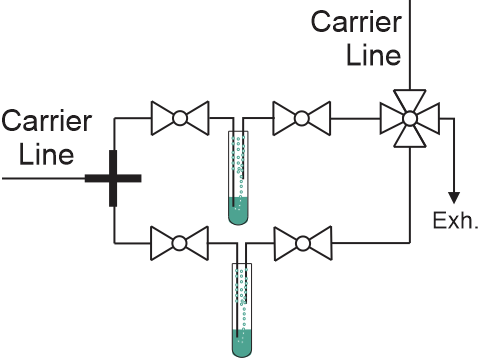
\includegraphics[width=0.5\textwidth,height=\textheight]{figures/ch9/multiplex-vapoursensor.png}

}

\caption{\label{fig-vapour-sensor-multiplexing}Multiplexing with a
second analyte bottle and four-way valve.}

\end{figure}

\cleardoublepage
\phantomsection
\addcontentsline{toc}{part}{Appendices}
\appendix

\hypertarget{vapour-system-hardware}{%
\chapter{Vapour System Hardware}\label{vapour-system-hardware}}

\hypertarget{tbl-vapour-sensor-components}{}
\begin{longtable}[]{@{}
  >{\raggedright\arraybackslash}p{(\columnwidth - 4\tabcolsep) * \real{0.5930}}
  >{\raggedright\arraybackslash}p{(\columnwidth - 4\tabcolsep) * \real{0.2209}}
  >{\raggedright\arraybackslash}p{(\columnwidth - 4\tabcolsep) * \real{0.1860}}@{}}
\caption{\label{tbl-vapour-sensor-components}Major components used in
construction of the vapour delivery system described in this
thesis.}\tabularnewline
\toprule\noalign{}
\begin{minipage}[b]{\linewidth}\raggedright
Description
\end{minipage} & \begin{minipage}[b]{\linewidth}\raggedright
Part No.
\end{minipage} & \begin{minipage}[b]{\linewidth}\raggedright
Manufacturer
\end{minipage} \\
\midrule\noalign{}
\endfirsthead
\toprule\noalign{}
\begin{minipage}[b]{\linewidth}\raggedright
Description
\end{minipage} & \begin{minipage}[b]{\linewidth}\raggedright
Part No.
\end{minipage} & \begin{minipage}[b]{\linewidth}\raggedright
Manufacturer
\end{minipage} \\
\midrule\noalign{}
\endhead
\bottomrule\noalign{}
\endlastfoot
Mass flow controller, 20 sccm full scale & GE50A-013201SBV020 & MKS
Instruments \\
Mass flow controller, 200 sccm full scale & GE50A-013202SBV020 & MKS
Instruments \\
Mass flow controller, 500 sccm full scale & FC-2901V & Tylan \\
Analogue flowmeter, 240 sccm max. flow & 116261-30 & Dwyer \\
Micro diaphragm pump & P200-B3C5V-35000 & Xavitech \\
Analogue flow controller, for micro diaphragm pump & X3000450 &
Xavitech \\
10 mL Schott bottle & 218010802 & Duran \\
PTFE connection cap system & Z742273 & Duran \\
Baseline VOC-TRAQ flow cell, purple & 043-950 & Ametek Mocon \\
Baseline VOC-TRAQ flow cell, red & 043-951 & Ametek Mocon \\
Humidity and temperature sensor & T9602-5-A & Telaire \\
Enclosure, for humidity and temperature sensor & MC001189 & Multicomp
Pro \\
\end{longtable}

\hypertarget{python-code-for-data-analysis}{%
\chapter{Python Code for Data
Analysis}\label{python-code-for-data-analysis}}

\hypertarget{code-repository}{%
\section{Code Repository}\label{code-repository}}

The code used for general analysis of field-effect transistor devices in
this thesis was written with Python 3.8.8. Contributors to the code used
include Erica Cassie, Erica Happe, Marissa Dierkes and Leo Browning. The
code is located on GitHub and the research group OneDrive, and is
available on request.

\hypertarget{sec-histogram-analysis}{%
\section{Atomic Force Microscope Histogram
Analysis}\label{sec-histogram-analysis}}

The purpose of this code is to analyse atomic force microscope (AFM)
images of carbon nanotube networks in .xyz format taken using an atomic
force microscope and processed in Gwyddion (see
\textbf{?@sec-afm-characterisation}). It was originally designed by
Erica Happe in Matlab, and adapted by Marissa Dierkes and myself for use
in Python. The code imports the .xyz data and sorts it into bins 0.15 nm
in size for processing. To perform skew-normal distribution fits, both
\emph{scipy.optimize.curve\_fit} and \emph{scipy.stats.skewnorm} modules
are used in this code.

\hypertarget{sec-raman-analysis}{%
\section{Raman Spectroscopy Analysis}\label{sec-raman-analysis}}

The purpose of this code is to analyse a series of Raman spectra taken
at different points on a single film (see
\textbf{?@sec-raman-characterisation}). Data is imported in a series of
tab-delimited text files, with the low wavenumber spectrum (100
cm\(^{-1} - 650\) cm\(^{-1}\)) and high wavenumber spectrum (1300
cm\(^{-1} - 1650\) cm\(^{-1}\)) imported in separate datafiles for each
scan location.

\hypertarget{sec-field-effect-transistor-analysis}{%
\section{Field-Effect Transistor
Analysis}\label{sec-field-effect-transistor-analysis}}

The purpose of this code is to analyse electrical measurements taken of
field-effect transistor (FET) devices. Electrical measurements were
either taken from the Keysight 4156C Semiconductor Parameter Analyser,
National Instruments NI-PXIe or Keysight B1500A Semiconductor Device
Analyser as discussed in \textbf{?@sec-electrical-characterisation}; the
code is able to analyse data in .csv format taken from all three
measurement setups. The main Python file in the code base consists of
three related but independent modules: the first analyses and plots
sensing data from the FET devices, the second analyses and plots
transfer characteristics from channels across a device, and the third
compares individual channel characteristics before and after a
modification or after each individual modification in a series of
modifications. The code base also features a separate config file and
style sheet which govern the behaviour of the main code. The code base
was designed collaboratively by myself and Erica Cassie over GitHub
using the Sourcetree Git GUI.

\hypertarget{references}{%
\chapter*{References}\label{references}}
\addcontentsline{toc}{chapter}{References}

\markboth{References}{References}

\printbibliography[heading=none]


\backmatter

\end{document}
